\documentclass[10pt,a4paper]{article}
\usepackage{amsmath}
\usepackage[margin=1in]{geometry}
\usepackage{amsmath}
\usepackage{amssymb}
\usepackage{color}
\usepackage{graphicx}
\usepackage{fancyhdr}
\usepackage{url}
%%%%%%%%%%%%%%%%%%%%%%%%%%%%%%%%%%%%%%%%%%%%%%%%%%%%%%
% lstlisting
%%%%%%%%%%%%%%%%%%%%%%%%%%%%%%%%%%%%%%%%%%%%%%%%%%%%%%
\usepackage{listings}             % Include the listings-package
\usepackage{alltt}
\definecolor{codegreen}{rgb}{0,0.6,0}
\definecolor{codegray}{rgb}{0.5,0.5,0.5}
\definecolor{codepurple}{rgb}{0.58,0,0.82}
\definecolor{backcolour}{rgb}{0.95,0.95,0.92}

\lstdefinestyle{mystyle}{
    backgroundcolor=\color{backcolour},
    commentstyle=\color{codegreen},
    keywordstyle=\color{codepurple},
    numberstyle=\tiny\color{codegray},
    stringstyle=\color{codepurple},
    basicstyle=\ttfamily\small,
    breakatwhitespace=false,
    breaklines=true,
    captionpos=b,
    keepspaces=true,
    numbers=left,
    numbersep=5pt,
    showspaces=false,
    showstringspaces=false,
    showtabs=false,
    tabsize=2,
    language=Fortran
}

\lstset{style=mystyle}

%%%%%%%%%%%%%%%%%%%%%%%%%%%%%%%%%%%%%%%%%%%%%%%%%%%%%%
% Graphs path to the Picture Folder
%%%%%%%%%%%%%%%%%%%%%%%%%%%%%%%%%%%%%%%%%%%%%%%%%%%%%%
\graphicspath{{Pictures/}{Data/}} % Two folders Picture and Data


\newcommand{\myUniversidad}{UNIVERSIDAD NACIONAL DEL CALLAO}
\newcommand{\myFacultad}{FACULTAD DE CIENCIAS NATURALES Y MATEM\'ATICA}
\newcommand{\myEscuelaProfesional}{ESCUELA PROFESIONAL DE F\'ISICA}
\newcommand{\myCurso}{F\'ISICA COMPUTACIONAL 2}
\newcommand{\myTarea }{Tarea }
\newcommand{\myNombre}{Tu nombre}
\newcommand{\myEmail}{email\_name@unac.gob,pe}
\newcommand{\myNumTarea}{1}

\pagestyle{fancyplain}
\lhead{\fancyplain{}{\textbf{Tarea \myNumTarea}}}      
\rhead{\fancyplain{}{\myNombre}}

%%%%%%%%%%%%%%%%%%%%%%%%%%%%%%%%%%%%%%%%%%%%%%%%%%%%%%
% bibliography
%%%%%%%%%%%%%%%%%%%%%%%%%%%%%%%%%%%%%%%%%%%%%%%%%%%%%%
%\usepackage{biblatex}
\bibliographystyle{plain}

%%%%%%%%%%%%%%%%%%%%%%%%%%%%%%%%%%%%%%%%%%%%%%%%%%%%%%
% Begin Document
%%%%%%%%%%%%%%%%%%%%%%%%%%%%%%%%%%%%%%%%%%%%%%%%%%%%%%
\begin{document}
%--------------------------------------------------------------------------------------------------
\thispagestyle{plain} % plain permite que la primera pagina no aparescan la barra en la parte superior de la pagina
%--------------------------------------------------------------------------------------------------
\begin{minipage}{.30\textwidth}
 
\includegraphics[width=.5\textwidth]{Escudo_UNAC.png}\\[.5cm]
\end{minipage}
\begin{minipage}{.65\textwidth}
 \begin{center}  % Center the following lines
\Large{                
\myUniversidad\\
\myFacultad\\ 
\myCurso\\
{\myTarea \myNumTarea}\\
\myNombre\\
\myEmail\\
\today}
\end{center} 
\end{minipage}\\
\centerline{\underline{\hspace{7in}}}
%\maketitle

\section*{Instrucciones}
Resuelva cuidadosamente cada problema. Si sudas, es normal. Si lloras, también. Asegúrate de incluir todos los pasos, unidades, diagramas (si aplica), y una pizca de paciencia. Si algo no cuadra... probablemente sea culpa del universo (o de las unidades mal convertidas).
\vspace{-1em}
\begin{center}
\textbf{Fuente:} Física Universitaria, Sears y Zemansky, 13ª Edición, Vol. 1 (2013), Capítulo 12, pág. 394
\end{center}

\vspace{1em}

% --- Repite este bloque para cada problema ---
\section*{Problema 1}
\textbf{Enunciado:} \\
Escribe aquí el enunciado del problema (o una versión resumida si lo tienes en el libro).

\vspace{1em}
\textbf{Solución:} \\

Aquí va la resolución paso a paso del problema.

\begin{itemize}
  \item Paso 1: Identificar qué demonios está pasando.
  \item Paso 2: Aplicar la ecuación correspondiente.
  \item Paso 3: Resolver, mantener la calma, y verificar unidades.
  \item Paso 4: Escribir la respuesta final con sus respectivas unidades.
\end{itemize}

% Puedes incluir una figura si es necesario
\begin{figure}[h]
\centering
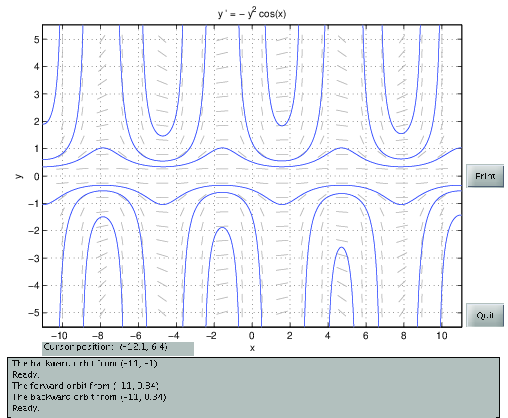
\includegraphics[width=0.5\textwidth]{fig1.png}
\caption{Diagrama esquemático del problema.}
\end{figure}

% Ejemplo de segundo problema
\section*{Problema 2}
\textbf{Enunciado:} \\
Escribe aquí el enunciado del problema (o una versión resumida si lo tienes en el libro). \cite{Ding_and_Williams}.\cite{Yang_Kurth_Willians}
%      \\\\
% Escribe aquí el enunciado
% ... \\\\
\textbf{Solución:} \\
\begin{equation}
  x_{n+1}  =  x_n - m\;f(x)\left[\frac{x_n-x_{n-1}}{f(x_n)-f(x_{n-1}}\right]
\end{equation}
\hspace{1mm}\\
For $m=\frac{1+\sqrt{5}}{2}=1.618$\\
\begin{verbatim}
Steps        xa              xb               xi           f(xi)       |(xn+1-xn)|
----------------------------------------------------------------------------------
  0  1.500000000000  1.600000000000  1.633191538329 -0.001945949763  0.033191538329 
  1  1.600000000000  1.633191538329  1.564416498720 -0.000020351034  0.068775039609 
  2  1.633191538329  1.564416498720  1.563240412447 -0.000028545785  0.001176086273 
  3  1.564416498720  1.563240412447  1.569869184045 -0.000000429797  0.006628771598 
  4  1.563240412447  1.569869184045  1.570033141259 -0.000000291226  0.000163957214 
  5  1.569869184045  1.570033141259  1.570590682342 -0.000000021145  0.000557541083 
  6  1.570033141259  1.570590682342  1.570661309883 -0.000000009115  0.000070627541 
  7  1.570590682342  1.570661309883  1.570747894571 -0.000000001173  0.000086584688 
  8  1.570661309883  1.570747894571  1.570768583633 -0.000000000385  0.000020689062 
  9  1.570747894571  1.570768583633  1.570784932394 -0.000000000065  0.000016348761 
 10  1.570768583633  1.570784932394  1.570790299953 -0.000000000018  0.000005367559 
 11  1.570784932394  1.570790299953  1.570793673498 -0.000000000004  0.000003373545 
 12  1.570790299953  1.570793673498  1.570794985787 -0.000000000001  0.000001312289 
 13  1.570793673498  1.570794985787  1.570795714281 -0.000000000000  0.000000728494 
\end{verbatim}
\begin{lstlisting}
! Codigo Fortran aqui
PROGRAM ejemplo
  IMPLICIT NONE
  INTEGER :: i, n
  REAL :: x, sum

  n = 100
  sum = 0.0

  DO i = 1, n
    x = REAL(i)
    sum = sum + x**2
  END DO

  PRINT *, 'La suma de los cuadrados es: ', sum

END PROGRAM ejemplo
\end{lstlisting}
%      \\\\
% Escribe aquí tu soluci\'on paso a paso. Puedes incluir ecuaciones, figuras, explicaciones y c\'odigo.
% ... \\\\

% ...y así sucesivamente hasta el problema 20


\begin{figure}[h]
    \centering
    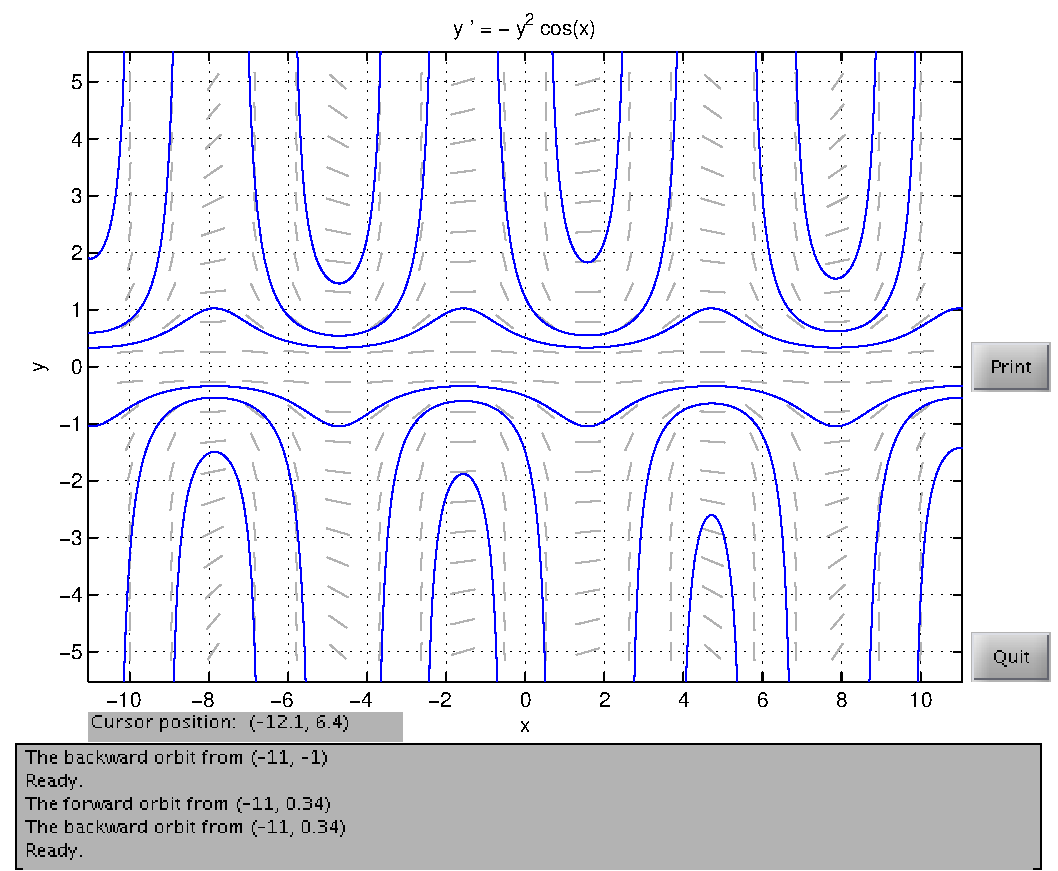
\includegraphics[width=0.5\textwidth]{fig2.pdf}
    \caption{Descripción de la figura}
\end{figure}

%%%%%%%%%%%%%%%%%%%%%%%%%%%%%%%%%%%%%%%%%%%%%%%%%%%%%%%%%%%%%%%%%%%%%%%%%%%%%%%%
%                                   Appendices page                            %                    
%%%%%%%%%%%%%%%%%%%%%%%%%%%%%%%%%%%%%%%%%%%%%%%%%%%%%%%%%%%%%%%%%%%%%%%%%%%%%%%%
\appendix
\addcontentsline{toc}{section}{Appendices}
\section*{Appendices}
\appendix
%\doublespacing
%\chapter{Appendix}

\section{Front-end and Back-end}
In software engineering, the terms \verb+front-end+ and \verb+back-end+ refer to the separation
of concerns between the presentation layer (\verb+front-end+), and the data access layer (\verb+back-end+) of a piece of software, 
or the physical infrastructure or hardware. Therefore in a HPC, 
\begin{itemize}
\item The login servers are called \verb+front-ends+ because you do not run your calculations there.
\item Rather run your calculations on \verb+back-end+ compute servers.
\item The \verb+front-end+ server provides access to compute servers via the \verb+batch+ system, using the \verb+qsub+ command.
\end{itemize}

\section{Hard Link or Symbolic Link}
The \verb+ln+ command is a \verb+Linux/Unix+ command used to create file links to an existing file. 
\subsection{Link types}
\begin{itemize}
\item There are two types of links
\begin{enumerate}
\item  \textbf{hard links:} Refer to the specific location of physical data.
A hard link allows multiple filenames to be associated with the same file since a hard link points to the 
inode of a given file, the data of which is stored on disk.
\item  \textbf{symbolic links:} Refer to a symbolic path indicating the abstract location of another file.
A symbolic links are special files that refer to other files by name.
\end{enumerate}
\item The \verb+ln+ command by default creates hard links, and when called with the command line parameter \verb+ln -s+
creates symbolic links.
\item Most operating systems prevent hard links to directories from being created since such a capability could disrupt
the structure of a file system and interfere with the operation of other utilities. 
\item The \verb+ln+ command can however be used to create symbolic links to  non-existent files. 
\end{itemize}

\subsection{Examples}
\begin{enumerate}
 \item Example 1
\begin{lstlisting}[language=bash,numbers=none] 
$ ln -s source_file target_file
\end{lstlisting}
\begin{lstlisting}[language=bash,numbers=none] 
$ ls -l source_file target_file
-rw-r--r--  1 veryv  wheel  0 Mar  7 22:01 source_file
lrwxr-xr-x  1 veryv  wheel  5 Mar  7 22:01 target_file -> source_file
\end{lstlisting} 
\item Example 2 - Create a symbolic link for \verb+/home/Desktop/Links/Example/example.cpp+ as \verb+/home/Test/example.cpp+,
copy paste the following command
\begin{lstlisting}[language=bash,numbers=none] 
$ ln -s   /home/Desktop/Links/Example/example.cpp    /home/Test/example.cpp
\end{lstlisting}
\begin{lstlisting}[language=bash,numbers=none] 
$ ll
lrwxrwxrwx 1 vivek  vivek    16 2007-09-25 22:53 example.cpp -> /home/Desktop/Links/Example/example.cpp
\end{lstlisting}
\end{enumerate}

\section{Securely Copy (SCP) Files}
\verb+SCP+ allows files to be copied to, from, or between different hosts (between a local host and a remote host or between two remote hosts.).
It uses \verb+ssh+ for data transfer and provides the same authentication and same level of security as \verb+ssh+.
\begin{enumerate}
 \item Copy the file \verb+foobar.txt+ from a remote host to the local host
\begin{lstlisting}[language=bash,numbers=none] 
$ scp your_username@remotehost.edu:foobar.txt /some/local/directory 
\end{lstlisting}
\item How to \verb+scp+ a file to LANL-IC \verb+turquoise/+
\begin{lstlisting}[language=bash,numbers=none] 
$ scp filename username@wtrw.lanl.gov:username@gr-fe.lanl.gov:/remote/path/to/file
\end{lstlisting}
\item Also shorter probably works
\begin{lstlisting}[language=bash,numbers=none] 
scp filename wtrw:gr-fe:/remote/path/to/file
\end{lstlisting}
\end{enumerate}

%%%%%%%%%%%%%%%%%%%%%%%%%%%%%%%%%%%%%%%%%%%%%%%%%%%%%%%%%%%%%%%%%%%%%%%%%%%%%%%%
%                  Bibliography  or References page                            %                    
%%%%%%%%%%%%%%%%%%%%%%%%%%%%%%%%%%%%%%%%%%%%%%%%%%%%%%%%%%%%%%%%%%%%%%%%%%%%%%%%      
% \newpage
%\nocite{*}
\bibliography{References/myBibliography}
\end{document}
